\documentclass[11pt]{article}

\usepackage[utf8]{inputenc}
\usepackage[T1]{fontenc}
\usepackage{amssymb}
\usepackage[a4paper, left=2cm, right=2cm, top=3.5cm, bottom=3.5cm]{geometry}
\usepackage[french]{babel}

% Paragraph spacing
\setlength{\parskip}{1em}

% Fancy headers
\usepackage{fancyhdr}

% Captions for subfigures
\usepackage{subcaption}

% Footnote inside a caption
\usepackage{fnpos}
\usepackage{ftnxtra}

% Maths
\usepackage{amsmath}

% Todo notes
\usepackage{todonotes}

% Table of contents for bibliography
\usepackage[nottoc]{tocbibind}

% Inline monospace font
\def\code#1{\texttt{#1}}

% Figures
\usepackage{graphicx}

% Draw figures
\usepackage{tikz}

% provides the H option
\usepackage{float}

% Tikz node rotation
\usetikzlibrary{positioning}

% Usage: \rotnode[options]{rotation}{text}
\newcommand\rotnode[3][]{%
    \node [#1, opacity=0.0] (tmp) {#3};
    \node [draw, rotate around={#2:(tmp.center)}] at (tmp) {#3};
}

% remove extra space
\newcommand{\squeezeup}{\vspace{-4.5cm}}

\usepackage{etoolbox}
\BeforeBeginEnvironment{figure}{\vskip-2ex}
\AfterEndEnvironment{figure}{\vskip-1ex}

% Clickable links
\usepackage{hyperref}

% Table of contents depth
\setcounter{tocdepth}{2}

% Inline code
\usepackage{listings}
\usepackage{color}

\title{Modélisation d'un jeu de données par une variable aléatoire}

\author{Othmane AJDOR}
\date{2018-2019}

\begin{document}
\maketitle

\pagebreak

\tableofcontents

\pagebreak

\section{Identificiation de modele}

\subsection{A : Temps de transfert de données entre 2 ordinateurs}
\begin{itemize}
    \item Loi normale (proche d'une valeur plus que les autres)
    \item Exponentielle décalée (dispositif sans usure)
    \item Support infini
\end{itemize}

\subsection{B : Nombre d'appel par heuere une hotline d'un FAI}
Loi de poisson.\\
C'est un cas discret, le nombre d'appel est un entier, donc ca peut pas etre exponentiel.

\subsection{C : Chiffre d'affaire annuel des entreprises clientes d'une banque}
Loi normale, on se place ici dans un interval $[-\infty,+\infty]$.


\subsection{D : Nombre de clients qu'il faut appeler avant d'en trouver un qui veut bien prendre 15' pour répondre à un questionnaire}
Loi géometrique

\subsection{E : Résultat d'un sondage sur des pieces sortant d'un chaine de production: sont elles aux normes ou pas ?}
Loi binomiale

\subsection{F : Poids d'une population de poulets âgés de 3 mois dans un elevage}
Loi normale

\subsection{G : Nombre de feux de circulation que l'on a au vert sur un parcours donné}
Loi binomiale, indépendance des feux, nombre de feux fixé.\\
Les feux ont les memes durées, soit le même p.

\subsection{H : Bruit de quantification sur 16 bits d'un signal sonore normalisé sur une plage $[-1,1]$}
Précision finie sur les bits (quantification).\\
Bruit de quantification = erreur causé par la quantification.
Continu de support limité.\\
Loi uniforme.

\subsection{I : Taille de défauts > à 20 mm sur la surface d'une cuve}
Loi exponentielle
Pour la taille des défauts, on commence à 20 et on regarde la taille des défauts supérieurs à 20mm.
On commence donc à un début d'intervale (ici $[20,+\infty]$). Or les défauts d'une taille de 10 metres par exemple sont quasi impossible.

Continu, support limité à partir de 20mm.
Loi normale tronquée.

Loi de parité

\subsection{J : Résultats d'un dé à 20 faces}
Loi uniforme discrete

\subsection{K : Nombre de pieces issues d'une chaine de production avant d'en trouver une defectueuse}
Loi géometrique

\pagebreak

\section{Méthodologie}
\subsection{Discret}
Pour des probabilités ou des valeurs qu'on peut compter, par exemple le lancé d'un dé
\subsection{Continu}
Sur des intervales infinis, par exemple le temps d'attente qu'un bus arrive ou le chiffre d'affaires des entreprises.

\subsection{Support}
Valeurs négatives?\\
Le dé à 20 faces est un support fini. Le nombre de feu rouges aussi.\\
Le poids ne peut pas etre négatif. Or la loi normale peut etre negative.\\
Or si on s'eloigne de quelques ecarts types, la proba tombre à 0.

\pagebreak

\section{Lois}
\subsection{Loi normale}
Les valeurs extremes n'ont pas de sens, par exemple le poids ou la taille de défauts.
Il existe beaucoup de facteurs qui peuvent changer le resultat.

\subsection{Loi exponentielle}
Pour la taille des défauts, on commence à 20 et on regarde la taille des défauts supérieurs à 20mm.
On commence donc à un début d'intervale (ici $[20,+\infty]$). Or les défauts d'une taille de 10 metres par exemple sont QUASI impossible.
Pour des durées de vie, pour des dispositifs sans usure.

\subsection{Loi de poisson}
Loi binomiale avec un n grand et un p tres petit ressemble à une loi de poisson.

\subsection{Loi géometrique}
Discrete, elle caracterise l'obtention d'un résultat positif apres une succession de tentatives, le cas du questionnaire.

\subsection{Loi bernoulli}
Cas spécial de la loi binamiale où $B(1,p) = B(p)$, soit n = 1.\\ 
Son résultat est binaire ($=1$ ou $=0$).

\subsection{Loi binomiale}
Somme de Bernoulli où on s'interesse à un ensemble de résultat au lieu d'un seul.

\pagebreak
\section{Recap des lois}
\squeezeup
\begin{figure}[h!]
    \centering
    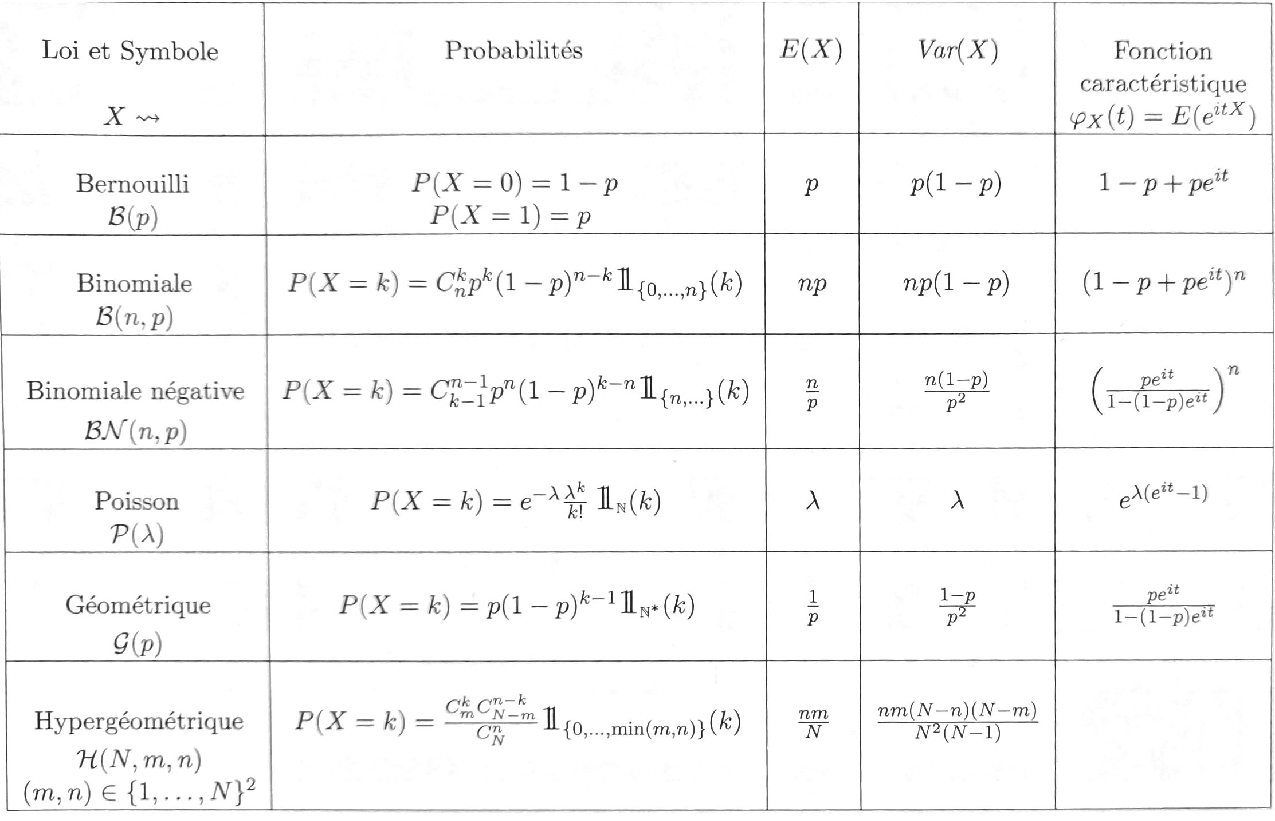
\includegraphics[scale=0.7]{img/recap.pdf}
\end{figure}

\end{document}